
%%%%%%%%%%%%%%%%%%%%%%%%%%%%%%%%%%%%%%%%%%%%%%%%%%
\chapter{ΒΑΣΙΚΕΣ ΕΝΝΟΙΕΣ ΧΡΟΝΟΣΕΙΡΑΣ}
%%%%%%%%%%%%%%%%%%%%%%%%%%%%%%%%%%%%%%%%%%%%%%%%%%%%%%%%%%%%%%%%%%%%%%%%%%%%%%%%%%%%
\section{ΓΕΝΙΚΑ ΠΕΡΙ ΠΡΟΒΛΕΨΕΩΝ}
%%%%%%%%%%%%%%%%%%%%%%%%%%%%%%%%%%

%%%%%%%%%%%%%%%%%%%%%%%%%%%%%%%%%%%%%%%%%%%%%
\section{Η ΕΝΝΟΙΑ ΤΗΣ ΧΡΟΝΟΣΕΙΡΑΣ}
%%%%%%%%%%%%%%%%%%%%%%%%%%%%%%%%%%%%%%%%%%%%%
 Η χρονοσειρά μπορεί να ορισθεί ως μια συλλογή διαδοχικών χρονικών
παρατηρήσεων της τιμής κάποιου μεγέθους. Πρόκειται ουσιαστικά για μια στοχαστική
διαδικασία, μιας και η εξέλιξη των τιμών του μεγέθους επηρεάζεται από τυχαίους
παράγοντες, ενώ η τιμή κάθε χρονικής στιγμής συνιστά και μια ξεχωριστή τυχαία
μεταβλητή. Με τον όρο χρονοσειρά δηλαδή, εννοούμε συνήθως μια ακολουθία $\{ x_t : t = 0,1,2,\ldots \}$ , όπου
κάθε $ x_t $ εκφράζει την κατά την χρονική στιγμή $ t $ κατάσταση ενός συστήματος το
οποίο εξελίσσεται στο χρόνο κατά τυχαίο εν γένει τρόπο (stochastic system).\\ 
Παραδείγματα τέτοιων χρονοσειρών είναι: \\
\begin{enumerate}


\item Οι ημερήσιες, αεροπορικές και οδικές, αφίξεις τουριστών στην χώρα μας $ x_t $ με
$t = 1, 2,\ldots $
\item Ο αριθμός $ x_t $ πελατών μέσα σε ένα πολυκατάστημα κατά τη χρονική στιγμή
$ t $ με $ t \in [0, T ] $.
\item Ο συνολικός αριθμός τροχαίων ατυχημάτων $ x_t $ κατά μήκος μιας οδικής
αρτηρίας στο χρονικό διάστημα [0,t] με t ≥ 0.
\item Η ημερήσια κατανάλωση ηλεκτρικού ρεύματος καθώς και η ημερήσια
κατανάλωση ύδατος, $ x_t $ και $ y_t $ αντίστοιχα, σε μια μεγάλη γεωγραφική περιοχή
της χώρας με $ t = 1, 2,\ldots $

\item Οι οικονομικές χρονοσειρές, όπως το ετήσιο ακαθάριστο εθνικό προϊόν και
ετήσιο ισοζύγιο εξωτερικών συναλλαγών $ x_t $ και $ y_t $ αντίστοιχα, με $ t = 1, 2,\ldots $
\item Οι μετεωρολογικές χρονοσειρές, όπως η θερμοκρασία περιβάλλοντος και
ατμοσφαιρική πίεση, $ x_t $ και $ y_t $ αντίστοιχα, σε συγκεκριμένη γεωγραφική
περιοχή με γεωγραφικές συντεταγμένες $ \left(l, a, h \right) $ κατά την χρονική στιγμή $ t $.
Εδώ η χρησιμοποιούμενη παράμετρος $ t $ είναι περισσότερο σύνθετη και
συγκεκριμένα $ t = \left( l,a,h ,t \right) $.
\end{enumerate}
%%%%%%%%%%%%%%%%%%%%%%%%%
%%%%%%%%%%%%%%%%%%%%%%%
%%%%%%%tha taa ksanadwwwwwwwwwww

Όπως διαπιστώνει κανείς από τα παραπάνω παραδείγματα, οι χρονοσειρές μπορούν
να αφορούν διακριτά μεγέθη $ x_t $ σε διακριτό χρόνο t, περίπτωση (i), διακριτά μεγέθη
$ x_t $ σε συνεχή χρόνο t, περιπτώσεις (ii) και (iii), συνεχή μεγέθη $x_t$ σε διακριτό χρόνο t, περιπτώσεις (iv) και (v) και συνεχή μεγέθη $x_t$ σε συνεχή χρόνο t, περίπτωση (vi).
Το πρόβλημα είναι η “πρόβλεψη” μελλοντικών τιμών της χρονοσειράς με βάση τις
μέχρι σήμερα τιμές τις ίδιας χρονοσειράς, περιπτώσεις (i)-(iii), είτε ακόμα και σε
συνδυασμό με τις μέχρι σήμερα τιμές μιας άλλης χρονοσειράς η οποία εξελίσσεται
παράλληλα με την πρώτη και επιδρά πάνω σ ́ αυτή, περιπτώσεις (iv)-(vi), οπότε
μιλάμε για πολυμεταβλητές χρονοσειρές. Το σύνολο των δυνατών καταστάσεων
ονομάζεται χώρος καταστάσεων και συμβολίζεται με S, ένα (μονοδιάστατο)
υποσύνολο του  $ R $   , ή γενικότερα ένα πολυδιάστατο υποσύνολο του $ R^d $, ενώ το
σύνολο τιμών του t ονομάζεται παραμετρικός χώρος, συμβολίζεται με Τ και μπορεί
επίσης να είναι υποσύνολο του $ R^k $, όταν χρειάζεται ένα πολυδιάστατο t για να
καθορίσουμε πέραν του χρόνου t και γεωγραφικές π.χ. συντεταγμένες $\left( l,a,h \right)$ σε
χωρο-χρονοσειρές (spatial time series), βλ. παράδειγμα (vi) παραπάνω. Σημειώνεται
οι όροι διακριτά και συνεχή μεγέθη είναι σε αντιστοιχία με τους όρους διακριτές και
συνεχείς τυχαίες μεταβλητές. \\ \\
Ένα παράδειγμα μίας χρονοσειράς απεικονίζεται στο ακόλουθο σχήμα 1.1, όπου παρουσιάζεται το γράφημα
της ετήσιας τιμής του αργού πετρελαίου σε αμερικανικά δολάρια ανά βαρέλι. Ο χρονικός ορίζοντας είναι 117 χρόνια, από το έτος 1870 έως το έτος 1987. Το γράφημα ελήφθη από το βιβλίο των R. Pindyck και
D. Rubinfeld (1998).\\\\
\begin{center}
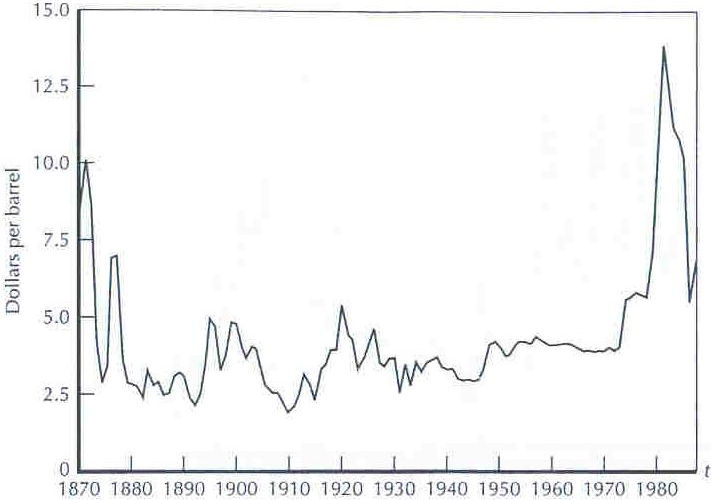
\includegraphics[scale=0.4]{graf1.png}\\   
\textbf{Σχήμα 1.1: Γράφημα χρονοσειράς τιμής αργού πετρελαίου σε δολάρια ανά βαρέλι.}
\end{center} 
\linespread{1}



Η συστηματική μελέτη μιας χρονοσειράς ξεκινάει με την επισκόπηση του
γραφήματός της στο πεδίο του χρόνου, από το οποίο μπορούν αρχικά να ανιχνευθούν
τρία βασικά ποιοτικά χαρακτηριστικά της: Η τάση, η εποχικότητα και οι ακραίες
παρατηρήσεις.\\
\begin{itemize}

\item Η \textbf{τάση} (trend) γενικά θα μπορούσε να ορισθεί ως η μακροπρόθεσμη μεταβολή του
μέσου επιπέδου των τιμών μιας χρονοσειράς. Έτσι, μπορεί η τάση των τιμών να είναι
αυξητική, πτωτική ή σταθερή σε ένα συγκεκριμένο χρονικό διάστημα, ενώ μπορεί και να
έχει τη μορφή κάποιας συνάρτησης στο εν λόγω διάστημα. Να σημειωθεί ότι η έννοια
“μακροπρόθεσμη μεταβολή” εξαρτάται από την εκάστοτε εφαρμογή που εξετάζεται.
\item Η \textbf{εποχικότητα} (seasonal) μπορεί να ορισθεί σαν μια περιοδική διακύμανση που έχει
σταθερό μήκος. Η εν λόγω διακύμανση τις περισσότερες φορές διακρίνεται εύκολα και
μπορεί να ερμηνευθεί στα πλαίσια του υπό μελέτη φαινομένου. Φερ' ειπείν, αν
κανείς επιθυμούσε να αναλύσει τη χρονοσειρά των τιμών των καυσίμων σε βάθος
χρόνων, είναι λογικό να περιμένει να παρατηρήσει μια σχετική άνοδο κατά τους
χειμερινούς μήνες κάθε έτους.

\item Οι \textbf{ακραίες παρατηρήσεις} (outliers) είναι οι απομονωμένες παρατηρήσεις που
εμφανίζονται στο γράφημα κάποιας χρονοσειράς ως απότομες αλλαγές στο πρότυπο
συμπεριφοράς της. Τα outliers μελετήθηκαν αρχικά κατά κύριο λόγο από τον A. J. Fox
(1972), ο οποίος μάλιστα εισήγαγε δύο τύπους. Ο τύπος I αφορά περιπτώσεις όπου η
ύπαρξη μιας ακραίας τιμής δεν έχει καμία επίδραση στις ακόλουθες παρατηρήσεις.
Αντιθέτως, ο τύπος ΙΙ αφορά περιπτώσεις όπου υπάρχει επίδραση στη μετέπειτα
συμπεριφορά των τιμών της χρονοσειράς, παράγοντας μια σειρά λιγότερο ή περισσότερο
ακραίων παρατηρήσεων ή αλλάζοντας εξ’ ολοκλήρου τα χαρακτηριστικά της.
\end{itemize}
Για την ανάλυση της χρονοσειράς εντοπίζουμε τα μοτίβα των διαθέσιμων δεδομένων
(δηλ, της χρονοσειράς) προκειμένου να καταλάβουμε τον τρόπο με τον οποίο
συμπεριφέρονται. Ακριβώς σε αυτή τη συμπεριφορά βασίζεται η πρόβλεψη. Αυτά τα
μοτίβα μπορεί να είναι:\\
\begin{enumerate}
%\begin{center}
%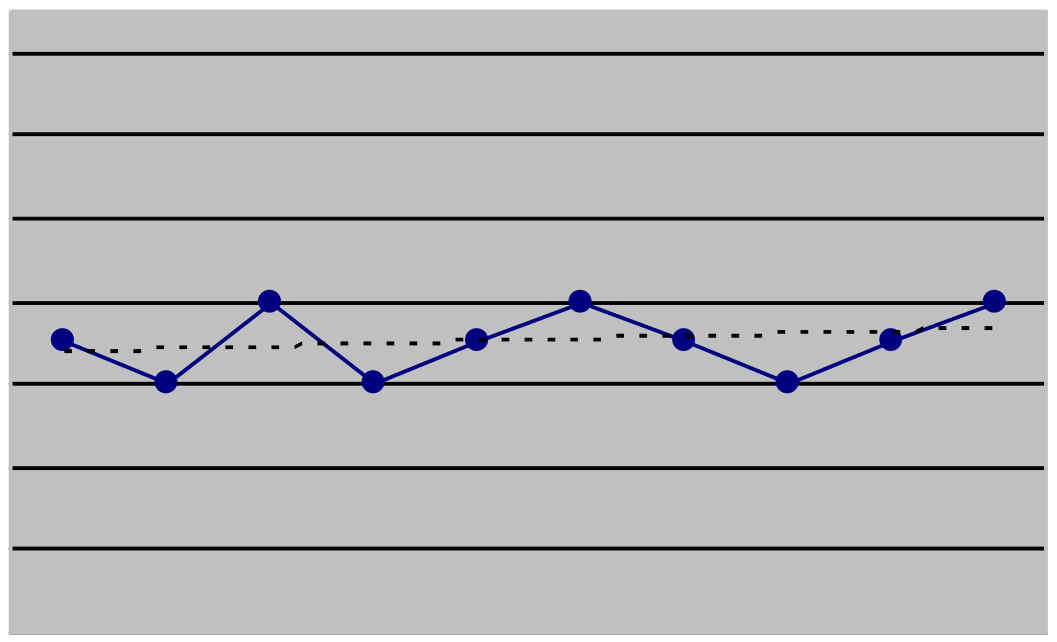
\includegraphics[scale=0.2]{level.png}\\
%\end{center}
\item τάση (trend): είναι η σταδιακή ανοδική ή πτωτική κίνηση των δεδομένων στο
χρόνο. Η κίνηση αυτή μπορεί να είναι γραμμική, εκθετική κτλ.\\
%\begin{center}
%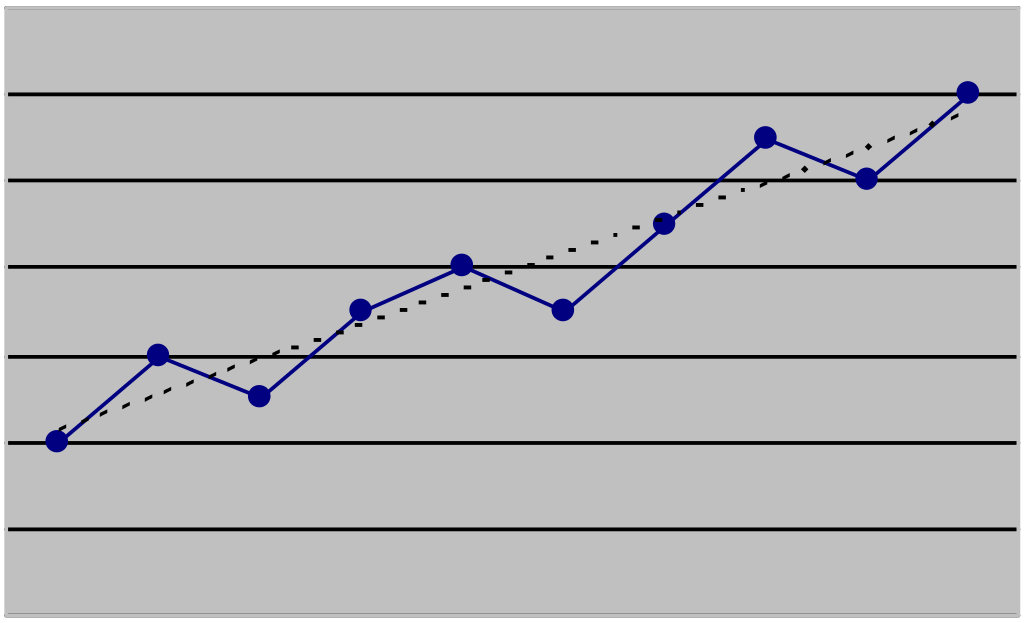
\includegraphics[scale=0.2]{trend.png}
%\end{center}
\item εποχικότητα (seasonality): είναι η κανονικά επαναλαμβανόμενη κίνηση των
δεδομένων μέσα σε σχετικά μικρό χρονικό διάστημα (συνήθως μέσα σε ένα
χρόνο). Τέτοιο μοτίβο μπορεί να παρουσιάζουν οι μεταβλητές που
επηρεάζονται από εποχικούς παράγοντες: π.χ. οι πωλήσεις παγωτών αυξάνουν
κατά τους ζεστούς μήνες και μειώνονται κατά τους κρύους.
%\begin{center}
%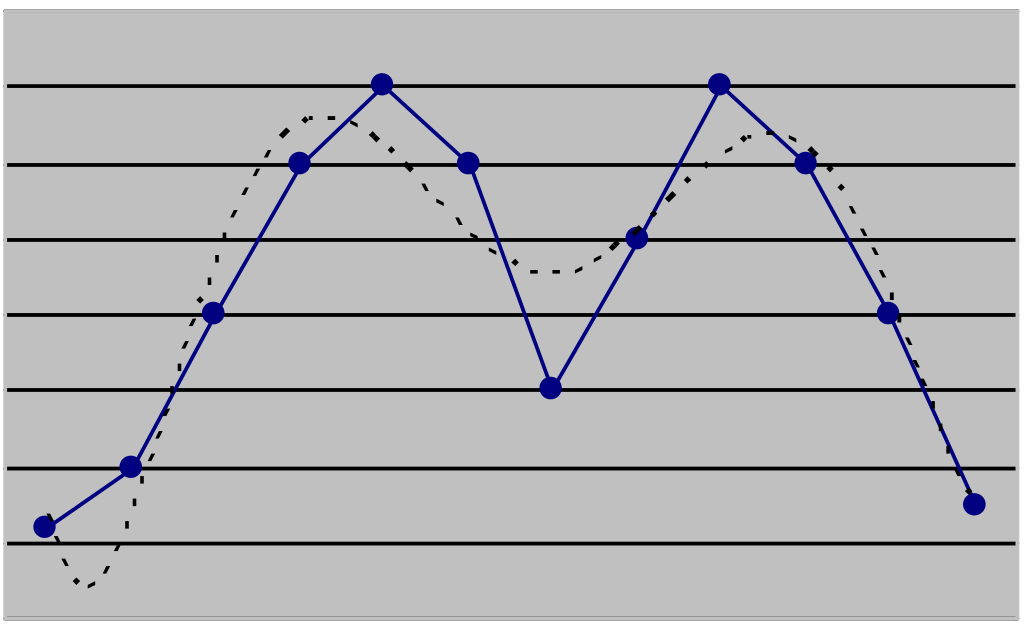
\includegraphics[scale=0.2]{season.png}
%\end{center}
\item κυκλικότητα (cycle): είναι (όπως και η εποχικότητα) η επαναλαμβανόμενη
αυξομείωση των δεδομένων, με μεγαλύτερο όμως χρονικό ορίζοντα (5-10
χρόνια), και είναι συνήθως συνδεδεμένη με τις διακυμάνσεις στο επίπεδο της
συνολικής οικονομίας (γνωστές ως περίοδοι οικονομικής ύφεσης και
οικονομικής ανάπτυξης).\\
%\begin{center}
%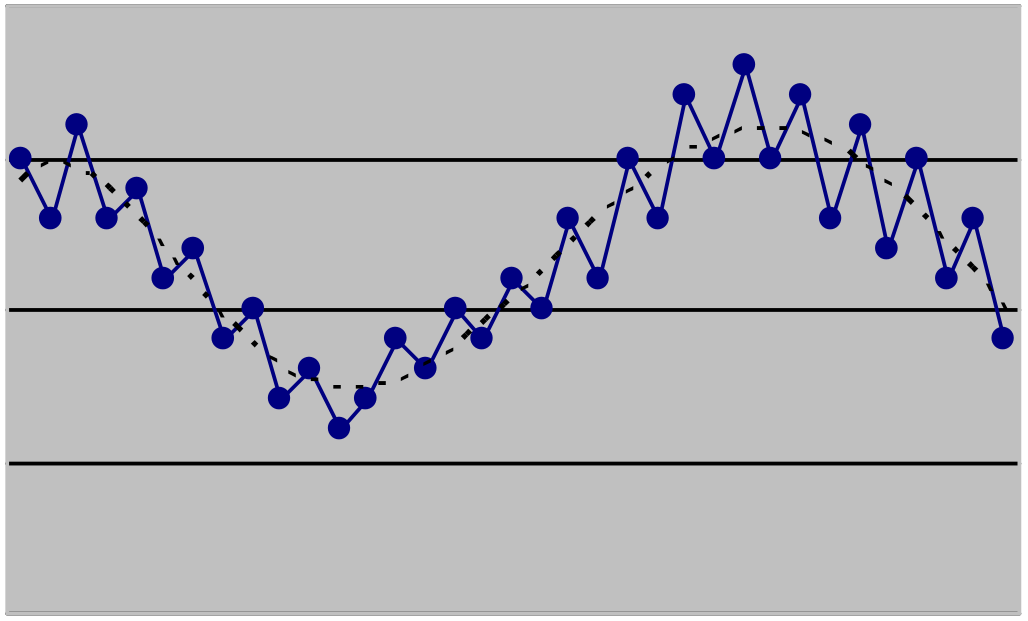
\includegraphics[scale=0.2]{cycle.png}
%\end{center} 
\item τυχαιότητα (randomness): είναι η κίνηση των δεδομένων που δεν παρουσιάζει
καμία κανονικότητα.
\end{enumerate}
%Αν εξετάσουμε μια οποιαδήποτε χρονοσειρά, διαπιστώνουμε ότι αποτελεί συνδυασμό
%ενός ή περισσότερων από τα παραπάνω στοιχεία.\\

\begin{center}
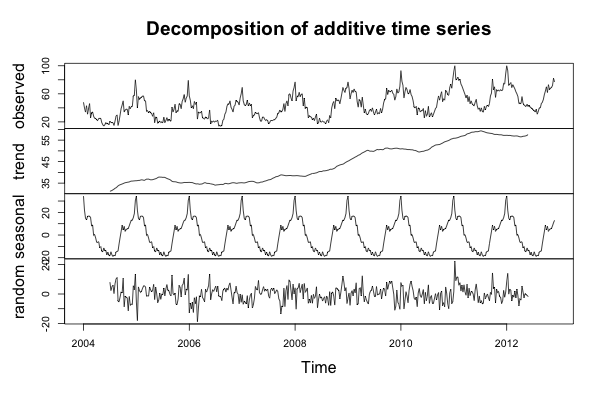
\includegraphics[scale=0.6]{pic2.png}
\end{center}
%%%%%%%%%%%%%%%%%%%%%%%%%%%%%%%%%%%%%%%%%%%%%%%
\section{ΠΑΡΑΔΕΙΓΜΑΤΑ ΠΡΑΓΜΑΤΙΚΩΝ ΧΡΟΝΟΣΕΙΡΩΝ}
%%%%%%%%%%%%%%%%%%%%%%%%%%%%%%%%%%%%%%%%%%%%%%%
Για να καταλάβουμε την σημαντικότητα της ανάλυσης χρονοσειρών είναι καλό
να δούμε κάποιες πραγματικές εφαρμογές και τα προβλήματα προς διερεύνηση. Κάποιες πραγματικές χρονοσειρές από διάφορα πεδία δίνονται στα ακόλουθα σχήματα. Τα
ερωτήματα μπορεί να διαφέρουν σε κάθε πεδίο αλλά το κοινό ζητούμενο είναι η
διερεύνηση της πληροφορίας που δίνει η χρονοσειρά.
\begin{center}
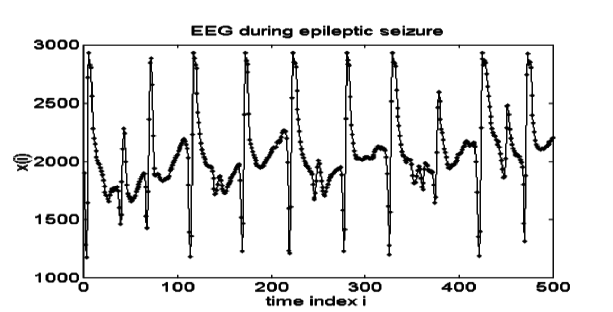
\includegraphics[scale=0.5]{graf5_1.png}\\
\textbf{Σχήμα 1.2: Ηλεκτροεγκεφαλογράφημα [EEG] από ένα ηλεκτρόδιο κατά τη διάρκεια επιληπτικής κρίσης.}
\end{center}
\begin{center}
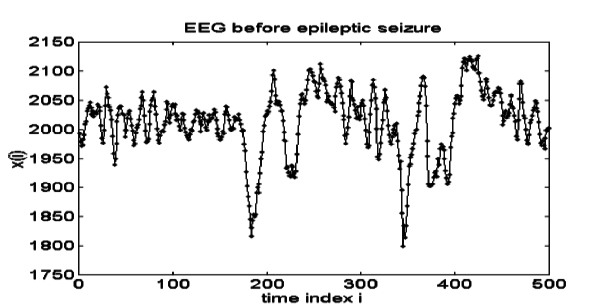
\includegraphics[scale=0.5]{graf5_2.png}\\
\textbf{Σχήμα 1.3: Ηλεκτροεγκεφαλογράφημα [EEG] πολύ πριν την κρίση.}
\end{center}
\begin{center}
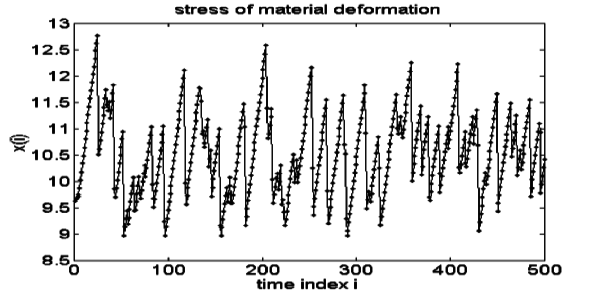
\includegraphics[scale=0.5]{graf5_3.png}\\
\textbf{Σχήμα 1.4: Συνολική Τάση κατά τη διάρκεια πειράματος παραμόρφωσης υλικού.}
\end{center}
\begin{center}
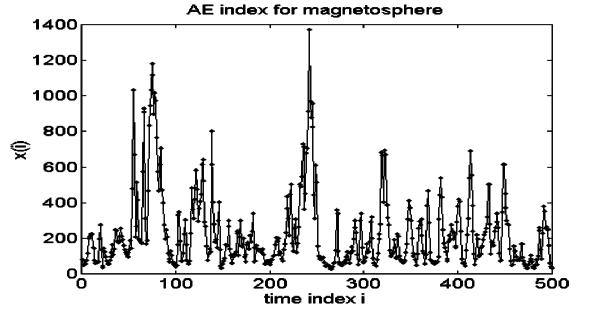
\includegraphics[scale=0.5]{graf5_5.png}\\
\textbf{Σχήμα 1.5: Δείκτης ΑΕ [aurora electrojet] για τη μαγνητική δραστηριότητα στο βόρειο πόλο. }
\end{center}
\begin{center}
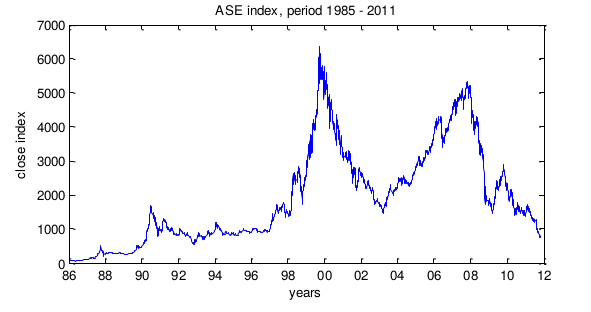
\includegraphics[scale=0.5]{graf5_6.png}\\
\textbf{Σχήμα 1.6: Ο Δείκτης του Χρηματιστηρίου Αξιών Αθηνών (ΧΑΑ) την περίοδο 1/1/1986-31/10/2011. }
\end{center}

%Μια από τις πιο γνωστές πραγματικές χρονοσειρές που έχουν μελετηθεί είναι η
%χρονοσειρά του πλήθους ηλιακών κηλίδων, δηλαδή μαύρων κηλίδων που
%εμφανίζονται στον ήλιο και μετά από κάποιο χρονικό διάστημα εξαφανίζονται.
%(Πιστεύεται πως ο αριθμός των ηλιακών κηλίδων επηρεάζει το κλίμα της γης) . Στο ακόλουθο σχήμα
%δίνεται η χρονοσειρά των ετήσιων ηλιακών κηλίδων από το 1700 ως το 2010.\\
\begin{center}
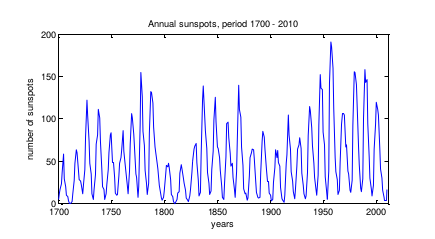
\includegraphics[scale=0.7]{graf5_7.png}\\
\textbf{ Σχήμα 1.7: Η χρονοσειρά των ετήσιων ηλιακών κηλίδων για την περίοδο 1700-2010.}
\end{center}
\begin{center}
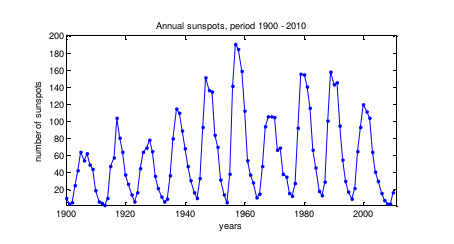
\includegraphics[scale=0.7]{graf5_8.png}\\
\textbf{Σχήμα 1.8: Η χρονοσειρά των ετήσιων ηλιακών κηλίδων για την περίοδο 1900-2010. }
\end{center}
%Όπως ήδη αναφέραμε, χρονοσειρά είναι μια ακολουθία τιμών
%$\{ x_t : t = 0,1,2,\ldots\}$ η οποία εκφράζει την εξέλιξη ενός στοχαστικού συστήματος, ενός
%συστήματος δηλαδή με τυχαία κατά μάλλον ή ήττον συμπεριφορά, σε αντίθεση με
%αυτήν ενός προσδιοριστικού (deterministic) συστήματος, η οποία συνήθως
%περιγράφεται από ένα σύστημα διαφορικών εξισώσεων. Όπως είναι γνωστό από την
%Θεωρία των Στοχαστικών Ανελίξεων, η εξέλιξη ενός στοχαστικού συστήματος
%μπορεί να περιγραφεί πιθανοθεωρητικά μέσω μιας στοχαστικής ανέλιξης (σ.α.),
%μονοδιάστατης ή πολυδιάστατης, δηλαδή μιας ακολουθίας τυχαίων μεταβλητών
%$\{X_n : n \in N \}$ , ή γενικότερα μιας (υπεραριθμήσιμης) οικογένειας τυχαίων
%μεταβλητών $\{X_t : t \in T \}$ , που ορίζεται πάνω σε ένα χώρο πιθανότητας $\left(\Omega , F , P \right)$ .
%
%Σημειώνεται ότι για δεδομένο $\omega \in \Omega$ , η $ \{x_t=X_t\left(\omega\right):t \in T\}$ εκφράζει μια
%συνάρτηση του χρόνου t και αποτελεί την τροχιά ή πραγματοποίηση (sample path,
%realization) της σ.α. $\{ X_t : t \in T \}$ . Συνεπώς, ο όρος χρονοσειρά
%χρησιμοποιείται τόσο για μια στοχαστική ανέλιξη $\{ X_t : t \in T \}$, όσο και για μία
%τροχιά $ \{x_t=X_t\left(\omega\right):t \in T\}$.

%%%%%%%%%%%%%%%%%%%%%%%%%%%%%%%%%%%%%%%%%%%%%%%%%%%%%%
\section{ΒΑΣΙΚΑ ΠΡΟΒΛΗΜΑΤΑ ΣΤΗΝ ΑΝΑΛΥΣΗ ΧΡΟΝΟΣΕΙΡΩΝ}
%%%%%%%%%%%%%%%%%%%%%%%%%%%%%%%%%%%%%%%%%%%%%%%%%%%%%%
Ο σκοπός της ανάλυσης χρονοσειρών μπορεί  να διαφέρει (π.χ. κατανόηση
του συστήματος, εκτίμηση διακριτικών χαρακτηριστικών του συστήματος,
πρόβλεψη), τα προβλήματα της ανάλυσης όμως είναι λίγο πολύ τα ίδια σε
πραγματικές εφαρμογές και έχουν να κάνουν με τη διαθέσιμη πληροφορία. Τα
κυριότερα προβλήματα σημειώνονται παρακάτω:

\begin{enumerate}
\item \textbf{Μονο-μεταβλητή χρονοσειρά}\\
Σε πολλά πραγματικά προβλήματα έχουμε
μετρήσεις ενός μόνο μεγέθους από το υπό μελέτη σύστημα, όπως για παράδειγμα
στο πείραμα πλαστικής παραμόρφωσης, όπου το μέγεθος που μετράμε είναι η
ολική τάση.
\item \textbf{Μια μόνο χρονοσειρά}\\
Σε χρονοσειρές από πειράματα, έχουμε τη δυνατότητα να
επαναλάβουμε το πείραμα και να πάρουμε μετρήσεις κάτω από τις ίδιες συνθήκες,
δηλαδή να παρατηρήσουμε περισσότερες από μια πραγματοποιήσεις του ίδιου
συστήματος. Ένα τέτοιο παράδειγμα είναι η χρονοσειρά ολικής τάσης από το
πείραμα πλαστικής παραμόρφωσης. Σε χρονοσειρές όμως από φυσικές
διαδικασίες, δεν υπάρχει αυτή η δυνατότητα καθώς δε μπορούμε να έχουμε
επαναλήψεις των μετρήσεων κάτω από τις ίδιες συνθήκες.
\item \textbf{Περιορισμένο μήκος χρονοσειράς}\\
Η αναζήτηση μεγάλων δειγμάτων είναι γνωστό
πρόβλημα στη στατιστική. Συχνά οι πραγματικές συνθήκες δεν το επιτρέπουν. Δε
μπορεί για παράδειγμα να ζητούμε μεγαλύτερη καταγραφή σε επιληπτική κρίση,
αφού η διάρκεια της είναι δεδομένη (και ευτυχώς σχετικά σύντομη), όπως δε
μπορούμε να έχουμε μετρήσεις του ημερήσιου δείκτη κλεισίματος ΧΑΑ πριν την
έναρξη του χρηματιστηρίου ή μετά τη σημερινή ημέρα.
\item \textbf{Ύπαρξη θορύβου}\\
Στα πραγματικά δεδομένα πάντα υπάρχει θόρυβος. Αυτός μπορεί να είναι δυναμικός ή θόρυβος συστήματος, έχει να κάνει δηλαδή με την
εξέλιξη του συστήματος και περιλαμβάνει όλες εκείνες τις εξωτερικές επιδράσεις
στο υπό μελέτη σύστημα που δε μπορούμε να εξηγήσουμε. Για παράδειγμα ο
δείκτης ΧΑΑ επηρεάζεται από άλλους χρηματο-οικονομικούς (και όχι μόνο)
παράγοντες που μπορούμε ενδεχομένως να συμπεριλάβουμε στη μελέτη μας
(πολύ-μεταβλητές χρονοσειρές), αλλά πάντα θα υπάρχουν και κάποιοι άλλοι
παράγοντες και τυχαία γεγονότα που επηρεάζουν την εξέλιξη του δείκτη ΧΑΑ και
δε μπορούμε να συμπεριλάβουμε, τα οποία αποτελούν το δυναμικό θόρυβο.
\item \textbf{Έλλειψη στασιμότητας}\\
Αυτό το πρόβλημα σχετίζεται με την ύπαρξη εξωτερικών
επιδράσεων ως προς το σύστημα που μελετάμε, που ενδεχομένως προσθέτουν
χαρακτηριστικά ξένα προς το σύστημα. Πολλές φορές το αποτέλεσμα είναι η
χρονοσειρά να παρουσιάζει μη-στασιμότητα, δηλαδή αργές μεταβολές (τάσεις) ή/και
περιοδικότητα, που δεν σχετίζονται με το μηχανισμό που θέλουμε να μελετήσουμε.
Για παράδειγμα, αν θέλουμε να διερευνήσουμε το μηχανισμό που καθορίζει τις
μεταβολές του ημερήσιου δείκτη από μέρα σε μέρα, δε μας ενδιαφέρει η στάθμη του
δείκτη, αν δηλαδή αναφερόμαστε στην περίοδο της λεγόμενης «φούσκας» του 2000 ή
της ύφεσης του 2011. Θα θέλαμε λοιπόν πρώτα να απαλείψουμε τις αργές μεταβολές
του δείκτη που έγιναν σε χρονικό ορίζοντα μηνών ή ετών.

\end{enumerate}
%Η ακολουθία των τυχαίων μεταβλητών $Y_t$ για κάθε χρονική στιγμή t ορίζει τη
%στοχαστική διαδικασία $ \{Y_t\}_{t=-\infty}^{+\infty}$(και αντίστοιχα για τη $X_t$ και $ \{X_t\}_{t=-\infty}^{+\infty}$ ). Θα
%αναφερόμαστε στη στοχαστική διαδικασία και ως χρονοσειρά εννοώντας την
%άγνωστη ακολουθία των τυχαίων μεταβλητών και όχι τις παρατηρήσεις. \\ \\
%Η πλήρης περιγραφή μιας στοχαστικής διαδικασίας $\{Y_t\}_{t=-\infty}^{+\infty} $ απαιτεί ότι οι κοινές
%κατανομές όλων των τάξεων
% είναι γνωστές για κάθε χρονική στιγμή t.
%Η κατανομή τάξης ένα αντιστοιχεί στη στατική περιγραφή της στοχαστικής
%διαδικασίας και είναι η (περιθώρια) κατανομή της $\{Y_t\}_{t=-\infty}^{+\infty} $\\
%$$ \forall t \in Z, \quad f_{Y_t}\left(y\right)=f_Y\left(y,t\right),$$
%δηλαδή ορίζεται ως συνάρτηση όχι μόνο της κάθε τιμής $y$ αλλά και του χρόνου t. Κατά τον ίδιο τρόπο η κοινή κατανομή δύο μεταβλητών της $\{Y_t\}_{t=-\infty}^{+\infty} $ (κατανομή τάξης
%2) είναι\\
%$$ \forall t_1,t_2 \in Z,\quad f_{Y_{t1},Y_{t2}} \left(y_1,y_2\right)= f_Y\left(y_1,y_2,t_1,t_2\right)$$.
%
%
%
%
%
%
%Δεδομένου ότι μια χρονοσειρά αποτελεί μια στοχαστική διαδικασία,
%δηλαδή κάθε παρατήρησή της αποτελεί μια τυχαία μεταβλητή,
%υποθέτουμε ότι μελετούμε την χρονική εξέλιξη των τιμών ενός μεγέθους $Υ$. Έτσι,
%την χρονική στιγμή t η τιμή του μεγέθους θα είναι μια τυχαία μεταβλητή $Y_t$ με
%συνάρτηση πυκνότητας πιθανότητας
%$f_{Y_t} \left(y_t \right)$. Έστω ακόμη ότι έχουμε παρατηρήσει ένα
%δείγμα τιμών μεγέθους Τ, δηλαδή έχουμε συλλέξει τις τιμές για $t = 1, 2,\ldots,T$
%$$\{ Y_1,Y_2,\ldots,Y_T \} $$
%
%Το παραπάνω δείγμα τιμών αναπαριστά μια συγκεκριμένη “έκβαση” της στοχαστικής
%διαδικασίας που γεννά τα δεδομένα. Αν τώρα η εν λόγω στοχαστική διαδικασία Υ
%επαναληφθεί Ν ανεξάρτητες φορές, θα έχουμε ένα σύνολο Ν “πραγματοποιήσεων” όλων
%των παρατηρήσεων – τυχαίων μεταβλητών $Υ_t$ που συνθέτουν τη χρονοσειρά. Συνεπώς,
%όσον αφορά το παραπάνω δείγμα τιμών μεγέθους Τ, για την κάθε μία παρατήρηση $Y_t$ θα
%έχουμε το εξής σύνολο\\
%$$ \{Y_t^{\left(1\right)},Y_t^{\left(2\right)},\ldots, Y_t^{\left(N\right)}\},\quad \forall t=1,2,\ldots,T$$
%
%%%%%%%%%%%%%%%%%%%%%%%%%%%%%%%%%%%%%%%%%%%%%%%%%%%%%%%%%%%%%%%%%%%%%
\section{ΣΤΟΧΑΣΤΙΚΗ ΔΙΑΔΙΚΑΣΙΑ ΚΑΙ ΚΑΤΗΓΟΡΙΕΣ ΧΡΟΝΟΛΟΓΙΚΩΝ ΣΕΙΡΩΝ}
%%%%%%%%%%%%%%%%%%%%%%%%%%%%%%%%%%%%%%%%%%%%%%%%%%%%%%%%%%%%%%%%%%%%%
Όπως ήδη έχουμε αναφέρει, η χρονοσειρά ή αλλιώς χρονολογική σειρά είναι μια σειρά από παρατηρήσεις που
παίρνονται σε ορισμένες χρονικές στιγμές ή περιόδους. Διαφορετικά, θα λέγαμε ότι 
είναι ένα δείγμα $ Y_1,Y_2,\ldots,Y_T $
όπου ο δείκτης παριστάνει ισαπέχοντα ή μη χρονικά
σημεία ή διαστήματα. Υποθέτουμε ότι οι παρατηρήσεις $ y_1,y_2,\ldots,y_T$
είναι
συγκεκριμένες τιμές ή συγκεκριμένες πραγματοποιήσεις των τυχαίων μεταβλητών $ Y_1,Y_2,\ldots,Y_T $
και ότι επιπλέον οι τυχαίες μεταβλητές αυτές
είναι μέρος
μιας άπειρης σειράς τυχαίων μεταβλητών. Η άπειρη αυτή ακολουθία των τυχαίων
μεταβλητών ονομάζεται στοχαστική ή τυχαία διαδικασία ή στοχαστική ανέλιξη και
παριστάνεται ως $ \{Y_t\}$.
 Με την ορολογία της κλασικής στατιστικής, η έννοια της
στοχαστικής διαδικασίας είναι ανάλογη της έννοιας του πληθυσμού, ενώ η έννοια της
συγκεκριμένης πραγματοποιήσεως είναι ανάλογη της έννοιας του δείγματος.\\

Γενικά, όπως και στην περίπτωση $T$ τυχαίων μεταβλητών, μια στοχαστική
διαδικασία μπορεί να περιγραφεί από μια συνάρτηση πιθανότητας $ f\left(y_1,y_2,\ldots,y_T\right). $
Εάν ήταν γνωστή η συνάρτηση πιθανότητας, τότε θα ήταν εύκολο να υπολογιστεί, για
παράδειγμα, η πιθανότητα μιας συγκεκριμένης πραγματοποιήσεως ή η πιθανότητα
μιας μελλοντικής τιμής. Επειδή όμως όχι μόνο η συνάρτηση πιθανότητας δεν είναι
γνωστή, αλλά ούτε και η πλήρης εξειδίκευση της μορφής της είναι δυνατή, σκοπός
της ανάλυσης χρονολογικών σειρών είναι η διατύπωση μοντέλων που να μπορούν να
περιγράψουν το μηχανισμό της στοχαστικής διαδικασίας από την όποια πρόεκυψε η
συγκεκριμένη χρονολογική σειρά.\\

Οι χρονολογικές σειρές διακρίνονται σε συνεχείς χρονολογικές σειρές και σε
διακριτές.\\\\
\textbf{ Συνεχείς  χρονοσειρές} (continuous) είναι αυτές όπου η τιμή του
φαινόμενου $ \left(X_t\right)$
παρατηρείται συνεχώς. Παράδειγμα συνεχών χρονολογικών σειρών
είναι η συνεχόμενη καταγραφή της θερμοκρασίας του αέρα ή η συνεχής
παρακολούθηση των σεισμών.\\

\begin{center}
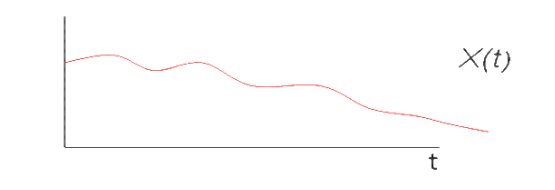
\includegraphics[scale=0.6]{graf6_1.png}
\textbf{Σχήμα 1.9: Συνεχής χρονολογική σειρά.}
\end{center}
\textbf{∆ιακριτές  χρονοσειρές} (discrete) είναι αυτές όπου η τιμή του
φαινομένου $ \left(X_t\right)$
καταγράφεται σε ορισμένα χρονικά διαστήματα $
\Delta t, t_i=i\Delta t.$

\begin{center}
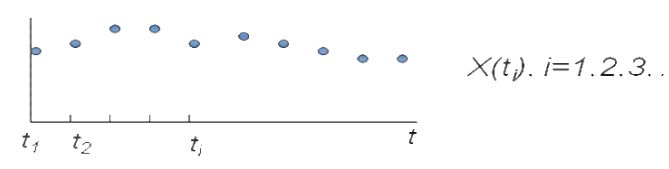
\includegraphics[scale=0.6]{graf6_2.png}
\textbf{Σχήμα 1.10: Διακριτή χρονολογική σειρά.}
\end{center}

Παράδειγμα διακριτών χρονολογικών σειρών είναι η τιμή μιας μετοχής ανά
ημέρα ή ο αριθμός των ηλιακών κηλίδων ανά έτος όπου υπάρχουν τιμές σε
συγκεκριμένα χρονικά διαστήματα.\\

Οι διακριτές χρονολογικές σειρές είναι αυτές που μπορούν να ‘κατανοηθούν’
από έναν Η/Υ. Συνεπώς, αντικειμενικός στόχος είναι οι συνεχείς χρονοσειρές να
μετατραπούν σε διακριτές. Η διαδικασία μετατροπής μιας συνεχούς χρονολογικής
σειράς σε διακριτή ονομάζεται διακριτοποίηση ή δειγματοληψία (Sampling, read off,
digitize) και είναι η διαδικασία κατά την οποία διαβάζοντας μια συνεχή χρονολογική
σειρά κρατάμε τιμές μόνο σε σημεία που απέχουν ορισμένη χρονική απόσταση $\Delta t$ ή
μετρώντας εξ αρχής μόνο σε διακριτές χρονικές στιγμές. Συνήθως αποφεύγεται μη
σταθερό $\Delta t$ καθώς δημιουργεί αρκετές δυσκολίες.\\
\begin{center}
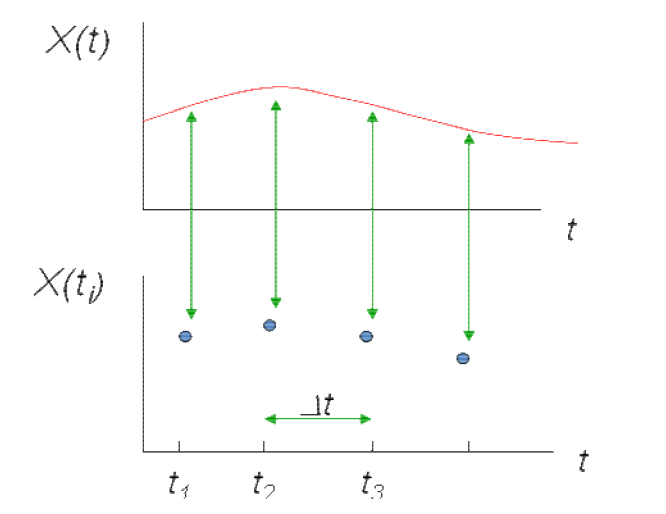
\includegraphics[scale=0.4]{graf7.png}\\
\textbf{Σχήμα 1.11: Μετατροπή Συνεχούς χρονολογικής σειράς σε ∆ιακριτή.}
\end{center}
Ορισμένες φορές στην διαδικασία μετατροπής μιας συνεχούς χρονολογικής σειράς σε
διακριτή είναι χρήσιμο να μην κρατιέται απλά η τιμή της συνεχούς χρονολογικής
σειράς στην χρονική στιγμή αυτή, αλλά το $ X\left(t_i\right)$
να είναι το άθροισμα ή το
ολοκλήρωμα για όλο το χρονικό διάστημα $ \Delta t$. Για παράδειγμα, όταν το $ X\left(t_i\right)$
είναι η βροχη σε $ mm^2 $ 
ανά ημέρα, λαμβάνεται το άθροισμα όλων των βροχοπτώσεων για κάποιο διάστημα, ή όταν το $ X\left(t_i\right)$
είναι η ραδιοακτινοβολία από τον ήλιο τότε σαν
$ X\left(t_i\right)$, λαμβάνεται\\
$$ X\left(t_i\right)=\frac{1}{\Delta t}\int_{t_{i-1}}^{t_i} f\left(t\right) dt $$
όπου $f\left(t\right) $ η συνεχής ακτινοβολία και $t_i-t_{i-1}=\Delta t. $\\

Στο σημείο αυτό πρέπει να σημειωθεί, ότι συνήθως στην ανάλυση
χρονολογικών σειρών οι διαδοχικές παρατηρήσεις δεν είναι ανεξάρτητες, άρα πρέπει
να λαμβάνεται υπ’ όψη η σειρά των παρατηρήσεων. Ακριβώς αυτή η εξάρτηση
επιτρέπει την πρόγνωση του μέλλοντος με βάση το παρελθόν.\\

Οι χρονολογικές σειρές εκτός από συνεχείς και διακριτές κατηγοριοποιούνται
σε ντετερμινιστικές, όπου επιτρέπουν την πρόγνωση με ακρίβεια και στοχαστικές
όπου επιτρέπουν προβλέψεις μόνο εν μέρει, δηλαδή με πιθανότητα p να συμβεί ένα
γεγονός.
%Η μέση τιμή (ροπή πρώτης τάξης) ή  αναμενόμενη τιμή $\mu_t$ της t–οστής παρατήρησης (τυχαίας μεταβλητής) $Y_t$
%της παραπάνω χρονοσειράς Υ δίδεται από τη σχέση:\\
%$$\mu = E \left[  Y_t \right]= \int_{-\infty }^{+\infty } y_tf_{Y_t}\left(y_t\right) dy   $$
%
%
%
%Η μέση τιμή $\mu_t$ σχετίζεται άμεσα
%με την έννοια της \textit{τάσης} της χρονοσειράς, εφόσον εκφράζεται ως συνάρτηση της
%χρονικής στιγμής $t$ της παρατήρησης $Y_t$ . Συγκεκριμένα, αν μια χρονοσειρά παρουσιάζει
%αυξητική ή πτωτική τάση αντιστοίχως σε ένα χρονικό διάστημα, αυτό θα αποτυπώνεται
%και στη μέση τιμή της $\mu_t$ ως συνάρτηση του χρόνου. Ακόμη, η μη ύπαρξη τάσης σε ένα
%χρονικό διάστημα αποτυπώνεται στη σταθερή αναμενόμενη τιμή $\mu_t$ στο εν λόγω
%διάστημα.
%
%\textbf{Η διασπορά}:\\ $$\sigma^2\left( t \right) =V \left[X_t \right] = E\left[\left( X_t-\mu_t\right) ^2  \right], \quad t \in T    $$
%
% \textbf{Η αυτοσυνδιακύμανση}:\\
%$$ \gamma\left(t,h \right) = Cov\left(X_t,X_{t+h} \right) =E\left[ \left(X_t-\mu_t \right)\left( X_{t+h}-\mu_{t+h}\right)  \right], \quad t,h \in T   $$ 
%
%Είναι προφανές ότι ισχύει: 
%$\sigma^2\left( t \right)=\gamma\left( t,0\right) =Cov\left(X_t,X_t \right),\quad t,h \in T   $ \\
%Είναι γνωστό επίσης ότι όταν οι διασπορές δύο τυχαίων μεταβλητών Χ και Υ , είναι
%πεπερασμένες, τότε τόσο οι μέσες τιμές αυτών όσο και η συνδιακύμανση αυτών
%είναι πεπερασμένες ποσότητες. Τούτο διότι αφενός πρέπει να έχουμε\\
%$E \left[ \vert X \vert ^2 \right]< ∞ , E \left[ \vert X \vert ^2 \right] < ∞ $, αφού διαφορετικά δεν ορίζονται οι διασπορές, και αφετέρου,
%με εφαρμογή της ανισότητας Cauchy-Schwarz\\
%$$E \left[\vert X \vert\vert Y \vert \right] \leq \sqrt{ E \left[ X^2 \right] E \left[ Y^2 \right]}, $$
%προκύπτει:\\
%$$\vert E \left[ X \right] \vert \leq E \left[\vert X \vert \right] \leq \sqrt{ E \left[ X^ 2 \right]} < ∞ , \quad \vert E \left[ Y \right] \vert \leq E \left[\vert Y \vert\right] \leq \sqrt{ E \left[ Y^ 2 \right]} < ∞  ,$$
%και
%$$ \vert Cov \left( X , Y \right) \vert \leq \sqrt{ V \left[ X \right] V \left[ Y \right]} < ∞ .$$


%\subsection{ΑΥΤΟΣΥΝΔΙΑΚΥΜΑΝΣΗ}
%\subsection{ ΑΥΤΟΣΥΣΧΕΤΗΣΗ}
%%%%%%%%%%%%%%%%%%%%%%%%%%%%%%%%%%%%%%%%%%%%%
\section{ΣΤΑΤΙΣΤΙΚΑ ΜΕΤΡΑ ΧΡΟΝΟΣΕΙΡΩΝ}
%%%%%%%%%%%%%%%%%%%%%%%%%%%%%%%%%%%%%%%%%%%%%

Άλλες βασικές έννοιες των χρονολογικών σειρών είναι η γραφική παράσταση,
ο μέσος όρος και η διασπορά αυτής, ο κινητό μέσος όρος, η τάση, η στασιμότητα και
άλλα.\\

Με την έννοια γραφική παράσταση μιας χρονολογικής σειράς εννοούμε την
καμπύλη που παράγεται σε ένα σύστημα ορθογωνίων αξόνων όπου ο οριζόντιος
άξονας είναι ο χρόνος και ο κατακόρυφος οι μετρούμενες τιμές στο αντίστοιχο
χρονικό διάστημα. Συμβολίζοντας με $ X_i $ τις $N$ χρονικές στιγμές και με $Y_i$ τις τιμές των
αντίστοιχων παρατηρήσεων, δημιουργούμε $N$ ζεύγη της μορφής $ \left(X_i,Y_i\right)$
όπου
μπορούμε να τα παραστήσουμε σε ένα σύστημα αξόνων.\\
\begin{center}
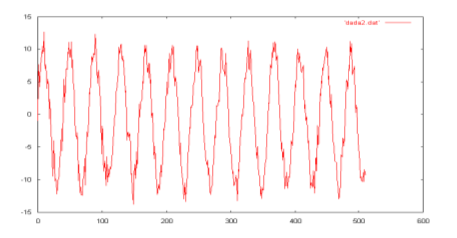
\includegraphics[scale=0.7]{graf8.png}\\
\textbf{Σχήμα 1.12: Γραφική παράσταση μιας τυχαίας χρονολογικής σειράς η οποία παρουσιάζει
περιοδικότητα. }
\end{center}
Με την βοήθεια της γραφικής παράστασης μιας χρονολογικής σειράς μπορούν
να γίνουν ορισμένες γρήγορες διαπιστώσεις. Στο παράδειγμα του σχήματος 1.12
βλέπουμε μια χρονοσειρά που δείχνει να είναι περιοδική με θόρυβο.\\\\
Έστω η χρονολογική σειρά $X\left(t_i\right),\: i=1,2,3,\ldots,N. $ \\
\textbf{ Μέσος όρος $\mu$} μιας χρονοσειράς είναι η μέση τιμή όλων των τιμών της. Όπως
γίνεται εύκολα αντιληπτό η σειρά των $X\left(t_i\right)$
δεν παίζει ρόλο.\\
$$ \mu=\frac{1}{N} \sum_{i=1}^{N} X\left(t_i\right).$$
\textbf{∆ιασπορά $\sigma^2$}
μιας χρονοσειράς είναι ο μέσος όρος των τετραγώνων των
αποκλίσεων από την μέση τιμή.\\
$$ \sigma^2=\frac{1}{N-1} \sum_{i=1}^{N} \left(X\left(t_i\right)-\mu\right)^2.  $$
%\begin{center}
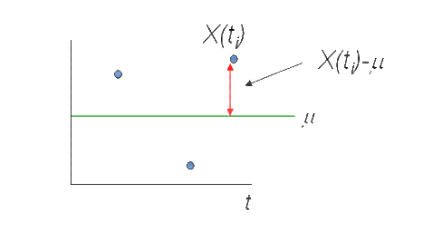
\includegraphics[scale=0.6]{graf9.png}\\
%\end{center}
\textbf{ Τυπική απόκλιση $ \sigma$} μιας χρονολογικής σειράς είναι η τετραγωνική ρίζα της
διασποράς.\\
$$ \sigma=\sqrt{\sigma^2}=\sqrt{\frac{1}{N-1}\sum_{i=1}^{N} \left(X\left(t_i\right)-\mu\right)^2}. $$
\begin{center}
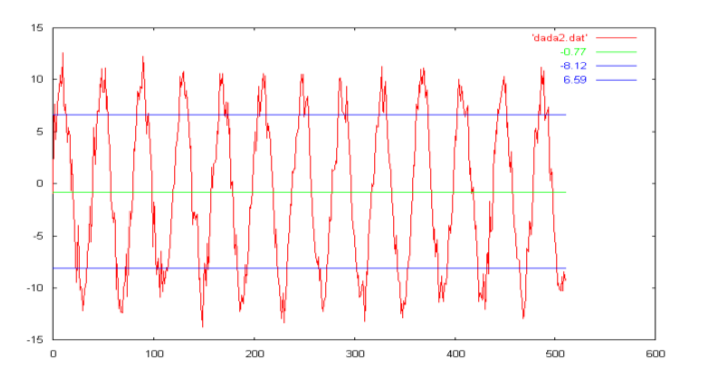
\includegraphics[scale=0.5]{graf10.png}\\
\textbf{Σχήμα 1.13: Γραφική παράσταση τυχαίας χρονολογικής σειράς, ο μέσος όρος και η τυπική
απόκλιση αυτής.}
\end{center}
Μεταξύ των τιμών $ \mu-\sigma$ και $\mu+\sigma$
βρίσκονται τα περισσότερα σημεία της
χρονολογικής σειράς. Το διάστημα αυτό δίνει και την διακύμανση των τιμών της
χρονολογικής σειράς. Υπάρχουν όμως χρονολογικές σειρές όπου τα μέτρα $ \mu$ και $ \mu\pm\sigma$
δεν δίνουν καλή περιγραφή της πραγματικής μέσης τιμής.\\
\begin{center}
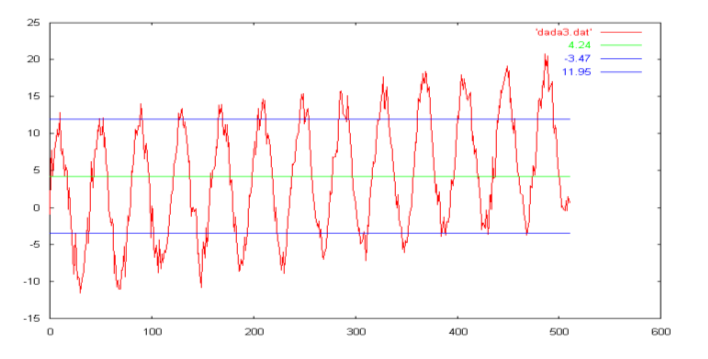
\includegraphics[scale=0.5]{graf11.png}\\
\textbf{Σχήμα 1.14: Γραφική παράσταση χρονολογικής σειράς, η οποία παρουσιάζει τάση.}
\end{center}
Ο λόγος έγκειται στο γεγονός πως υπάρχει μια τάση και έτσι η πραγματική μέση τιμή
μ αλλάζει με τον χρόνο, δηλαδή η μέση τιμή είναι συνάρτηση του χρόνου $ \mu=\mu\left(t\right).$
Έτσι, υπάρχει η ανάγκη να κατασκευαστεί ένα μοντέλο για την τάση. Ο πρώτος
τρόπος για την κατασκευή αυτού του μοντέλου είναι να δεχτούμε αυθαίρετα ότι η
τάση ακολουθεί κάποια γνωστή κατανομή. Στο σχήμα 1.14, σαν μια πρώτη προσέγγιση
μπορούμε να δεχθούμε ότι η μέση τιμή μεταβάλλεται γραμμικά ως προς τον χρόνο
$ \mu\left(t\right)=\alpha+bt.$\\
Συστηματοποιώντας την διαδικασία κατασκευής μοντέλου για την τάση κατασκευάστηκε ο κινητός μέσος όρος (running mean, moving average).\\
\begin{center}
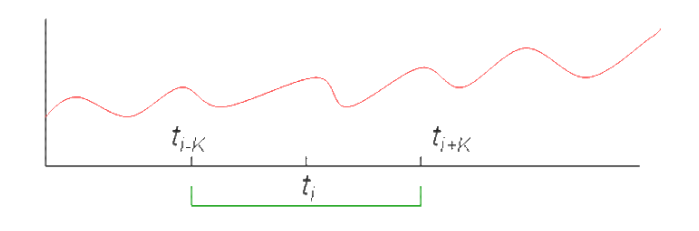
\includegraphics[scale=0.5]{graf12.png}\\
\end{center}
Έτσι, σαν κινητό μέσο όρο ορίζουμε\\
$$ \mu\left(t_i,K\right):=\frac{1}{2K+1} \sum_{j=i-K}^{i+K} X\left(t_j\right)$$
Στο ακόλουθο σχήμα 1.15 φαίνεται ο κινητός μέσος
όρος όπως αυτός ορίστηκε.\\
\begin{center}
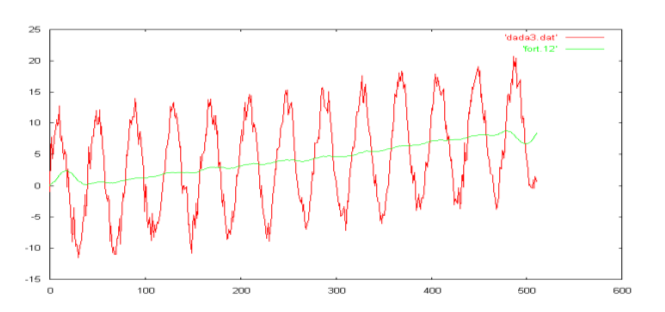
\includegraphics[scale=0.5]{graf13.png}\\
\textbf{Σχήμα 1.15: Ο κινητός μέσος όρος για τυχαία χρονολογική σειρά.}
\end{center}

Στις χρονοσειρές δεν υπάρχουν μόνο περιπτώσεις με την συμπεριφορά της τάσης όπως παραπάνω. Εκτός, λοιπόν, από την μακροχρόνια τάση (Secular
Trend), στις χρονολογικές σειρές συναντάμε είτε κυκλική κύμανση αυτών, είτε
περιοδική- εποχιακή μεταβολή, είτε ακανόνιστη μεταβολή. Συνήθως, στην πράξη
συναντάμε περισσότερα από ένα χαρακτηριστικά.\\\\
Στην μακροχρόνια τάση η τιμή της μεταβλητής τείνει να αυξηθεί ή να
ελαττωθεί για μεγάλο χρονικό διάστημα.
\begin{center}
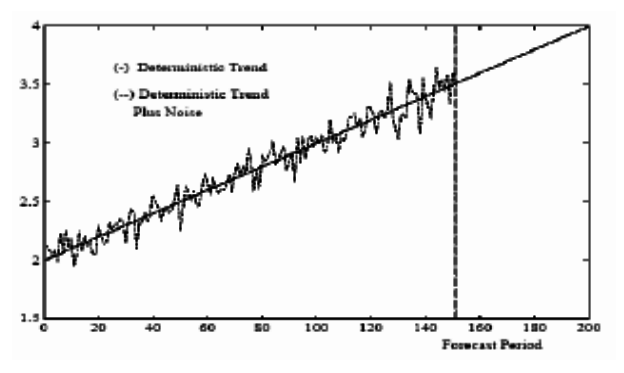
\includegraphics[scale=0.5]{graf14.png}\\
\textbf{Σχήμα 1.16: Xρονοσειρά που παρουσιάζει μακροχρόνια τάση.}
\end{center}

Η μακροχρόνια τάση είναι από τις περισσότερο εύκολα αντιμετωπίσιμες
περιπτώσεις γιατί η τάση εκφράζει την χρονολογική σειρά για μια εκτεταμένη
περίοδο. Οι χρονοσειρές που παρουσιάζουν μακροχρόνια τάση είναι αυτές που έχουν μελετηθεί περισσότερο. Επίσης, στις χρονοσειρές με μακροχρόνια
τάση είναι εύκολη η κατανόηση της ιστορίας της μεταβλητής με συνέπεια την
πρόβλεψη μελλοντικών τιμών. Ορισμένες μέθοδοι προσδιορισμού της μακροχρόνιας
τάσης είναι η μέθοδος των δυο μέσων σημείων, η μέθοδος των κινητών μέσων, η
μέθοδος της ευθείας ελαχίστων τετραγώνων, η μέθοδος της καμπύλης ελαχίστων τετραγώνων και άλλα.\\

Η κυκλική κύμανση που παρουσιάζουν περιπτώσεις χρονοσειρών έγκειται στο γεγονός ότι παρατηρούνται αυξομειώσεις της τιμής της μεταβλητής
γύρω από γραμμή τάσης σε μια μακροχρόνια περίοδο. Στην πράξη τα σημεία της
χρονοσειράς για μια χρονική σειρά παρατηρήσεων βρίσκονται κάτω από την
γραμμή τάσης και στην συνέχεια για άλλη χρονική σειρά τιμών πάνω από την γραμμή
τάσης. Ο χρόνος για να έχουμε μια κυκλική αυξομείωση δεν είναι σταθερός.
\begin{center}
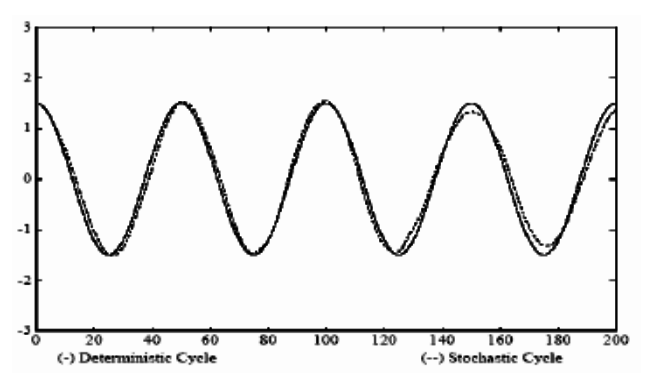
\includegraphics[scale=0.5]{graf15.png}\\
\textbf{Σχήμα 1.17: Xρονοσειρά που παρουσιάζει κυκλική κύμανση.}
\end{center}
Στην πράξη οι κυκλικές αυξομειώσεις είναι οι πλέον δύσκολες να αντιμετωπιστούν γιατί η κυκλική κίνηση δεν ακολουθεί κανένα κανονικό μοντέλο
αλλά κινείται απρόβλεπτα.\\

Αντίθετα, από τις χρονολογικές σειρές που παρουσιάζουν κυκλικές μεταβολές
και είναι δύσκολα αντιμετωπίσιμες, οι χρονολογικές σειρές που παρουσιάζουν
περιοδικές μεταβολές είναι πολύ χρήσιμες γιατί ακολουθούν κανονικό μοντέλο και
έτσι μπορούν να δώσουν αξιόπιστες προβλέψεις για το μέλλον.
\begin{center}
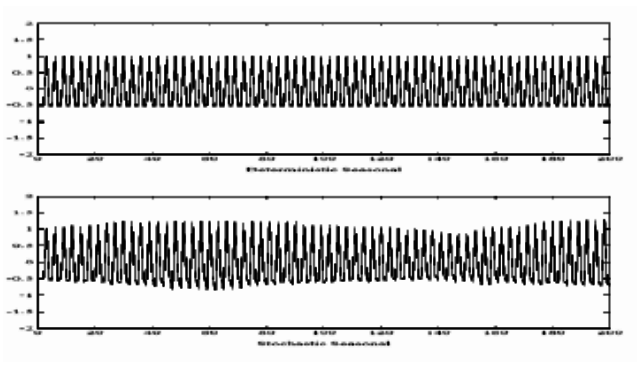
\includegraphics[scale=0.5]{graf16.png}\\
\textbf{Σχήμα 1.18: Xρονοσειρά που παρουσιάζει περιοδικότητα.}
\end{center}

Τέλος, υπάρχουν και χρονοσειρές που παρουσιάζουν ακανόνιστες μεταβολές, μεταβολές που άλλοτε είναι μικρές, άλλοτε μεγάλες, θετικές ή αρνητικές
χωρίς καμία κανονικότητα. Οι μεταβολές αυτές διακρίνονται σε συμπτωματικές,
οφειλόμενες σε απρόβλεπτα γεγονότα και τυχαίες.
%%%%%%%%%%%%%%%%%%%%%%%%%%%%%%%%%%%%%%%%%%%%%
\section{ΣΤΑΣΙΜΟΤΗΤΑ}
%%%%%%%%%%%%%%%%%%%%%%%%%%%%%%%%%%%%%%%%%%%%%
Η στασιμότητα είναι πολύ σημαντική έννοια καθώς είναι απαραίτητη προϋπόθεση για τα περισσότερα εργαλεία της ανάλυση χρονολογικών σειρών.\\

Όπως έχει ήδη αναφερθεί,η χρονολογική σειρά μπορεί να θεωρηθεί ως στοχαστική
διαδικασία πεπερασμένου πλήθους παρατηρήσεων, δηλαδή την πραγματοποίηση μιας διαδικασίας $ X_1,X_2,\ldots,X_T.$ Για να ορίσουμε ένα μοντέλο χρονοσειρών, για ένα σύνολο παρατηρήσεων $\{x_t\} $
απαιτείται ο καθορισμός όλων των κοινών κατανομών μιας ακολουθίας $ X_t$, πραγματοποίηση των οποίων πρέπει να είναι οι παρατηρήσεις $\{x_t\}. $ Η
αναζήτηση λοιπόν ενός μοντέλου, συνεπάγεται τον ορισμό όλων των κοινών κατανομών των $ X_1,X_2,\ldots,X_n$ με $n=1,2,\ldots$ δηλαδή των πιθανοτήτων \\
$ P \left( X_1 \leq x_1,X_2 \leq x_2, \ldots,X_T\leq x_n \right) $ 
με $\infty \leq  x_1 \leq x_2 \leq \ldots \leq x_n \leq \infty \:\: n=1,2,\ldots$
μια διαδικασία η όποια είναι εξαιρετικά δύσκολη. Στη θέση της ορίζονται και χρησιμοποιούνται ροπές μικρότερης τάξης. Βασική και απαραίτητη υπόθεση ώστε να απλοποιηθούν σημαντικά προβλήματα που προκύπτουν από την μελέτη των ροπών είναι η υπόθεση της στασιμότητας.\\

Προτού, οριστεί πλήρως μαθηματικά η στασιμότητα, γίνεται μια προσπάθεια να δοθεί ένας πρώτος διαισθητικός ορισμός. Μια χρονολογική σειρά λέγεται στάσιμη εάν δεν υπάρχει συστηματική αλλαγή του μέσου όρου και της διασποράς της στο
χρόνο. Με άλλα λόγια, εάν μια χρονοσειρά παρουσιάζει τάση τότε αυτή δεν θα είναι στάσιμη.\\

Μια στοχαστική διαδικασία είναι αυστηρώς ή πλήρως στάσιμη (strictly – strongly – completely stationary) όταν οι ιδιότητες της δεν επηρεάζονται από μια αλλαγή στην αρχή μετρήσεως του χρόνου.
Συνήθως, οι διαδικασίες αυτές λέγονται και n–τάξης στάσιμες. Αυτό σημαίνει ότι 
$$ F\left( y_t,y_{t+1},\ldots ,y_{t+T}\right)=F\left(y_{t+s},y_{t+1+s}, \ldots,y_{t+T+s}\right) $$
για οποιοδήποτε s, δηλαδή η από κοινού συνάρτηση κατανομής με αρχή το χρονικό σημείο t είναι η ιδία με την από κοινού συνάρτηση κατανομής με αρχή το χρονικό σημείο $t+s$. Το s παριστάνει μια
αυθαίρετη μετακίνηση κατά μήκος του άξονα του χρόνου είτε προς τα εμπρός είτε προς τα πίσω. Ο αυστηρός όμως, ορισμός της στασιμότητας αναφέρεται σε όλες τις ιδιότητες μιας στοχαστικής διαδικασίας. Πράγμα αρκετά δύσκολο. Αδυνατίζοντας τον ορισμό για την στασιμότητα, παράλληλα όμως μετατρέποντάς τον σε
περισσότερο ευέλικτο, ορίζεται η n-τάξεως ασθενώς στάσιμη διαδικασία εάν
υπάρχουν οι ροπές n-τάξεως και είναι ανεξάρτητες του t. ∆ηλαδή, εάν ισχύουν τα εξής:\\

$E \left(Y_t\right)=\mu,\:$ ανεξάτητη του t,\\

$Var \left(Y_t \right) = \sigma^2,\:$ ανεξάρτητη του t,\\

$Cov\left(Y_t,Y_{t+s}\right)=Cov\left(Y_{t+m},Y_{t+s+m}\right)=\gamma_s,\:$ ανεξάρτητη του t $\quad  \quad \: \left( A \right)$\\
$\quad \:$ κ.ο.κ.\\
Όταν οι παραπάνω συνθήκες περιορίζονται και αναφέρονται μόνο στις πρώτες και δευτέρες ροπές μιλάμε για 2-ης τάξης ασθενώς στάσιμες διαδικασίες ή απλώς ασθενώς
στάσιμες διαδικασίες ή κατά συνδιακύμανση στάσιμες.\\

Από την σχέση $ \left( A \right)$ είναι προφανές ότι $ Cov \left( Y_t,Y_{t+s}\right)=Cov \left(Y_{t+s},Y_t\right) $ δηλαδή $\gamma_s=\gamma_{-s}$. Επειδή $ Y_t $ και $ Y_{t+s} $ είναι παρατηρήσεις της ίδιας μεταβλητής που απέχουν χρονικά μεταξύ τους κατά s, η συνδιακύμανση $ Cov \left( Y_t,Y_{t+s}\right)$
αναφέρεται και ως αυτοσυνδιακύμανση. Είναι προφανές ότι για $ s=0,\: \gamma_0 = Var \left(Y_t \right)= \sigma^2.$ Τέλος, εάν
μια χρονολογική σειρά είναι αυστηρά στάσιμη τότε θα είναι και ασθενώς στάσιμη 2-ης
τάξης.

%Η στατιστική περιγραφή της στοχαστικής διαδικασίας απλουστεύεται αν
%θεωρήσουμε ότι οι στατιστικές της ιδιότητες παραμένουν σταθερές στο χρόνο και
%τότε η στοχαστική διαδικασία ορίζεται ως στάσιμη. Αυτή είναι μα υπόθεση που
%δύσκολα μπορεί να υιοθετηθεί σε πολλά πραγματικά προβλήματα, αλλά μπορεί να
%χρησιμοποιηθεί ως υπόθεση εργασίας για την εξαγωγή χρήσιμων συμπερασμάτων.\\ \\
%Ειδικότερα ορίζονται δύο μορφές στασιμότητας:\\


%Η ύπαρξη μη-στασιμότητας είναι ένα από τα βασικότερα προβλήματα στην
%ανάλυση χρονοσειρών.

%Είναι φανερό ότι έχοντας παρατηρήσει μια χρονοσειρά
%$ \{ X_t : t \in T \} $
%από κάποια
%χρονική στιγμή $ t = 0 $, έστω μέχρι και την παρούσα χρονική στιγμή $ t = s $, αν δηλαδή
%γνωρίζουμε την τροχιά αυτής $ \{ X_t : 0 \leq t \leq s \}$ , και θέλουμε να προβλέψουμε
%μελλοντικές τιμές αυτής $ X_{s + h} $, με $ h > 0 $, θα πρέπει να βασιστούμε στις μέχρι τώρα
%γνωστές τιμές της και στην εξάρτηση που ενδέχεται να υπάρχει μεταξύ $ X_{s + h} $ και
%των τιμών
%$ \{ X_t : 0 \leq t \leq s \}$
%της χρονοσειράς στο παρελθόν. Τούτο βέβαια με την
%προϋπόθεση ότι όλα τα πιθανοθεωρητικά χαρακτηριστικά μιας χρονοσειράς, ή
%τουλάχιστον τα βασικότερα εξ αυτών, παραμένουν αναλλοίωτα στον χρόνο. \\ \\
%Όταν όλα τα πιθανοθεωρητικά χαρακτηριστικά μιας χρονοσειράς παραμένουν
%αναλλοίωτα στο χρόνο τότε μιλάμε για \textit{αυστηρή στασιμότητα}. Συγκεκριμένα έχουμε:
%\begin{enumerate}
%\begin{dinglist}{43}
%\item \textbf{ Αυστηρή Στασιμότητα} \\\\
%Η στοχαστική διαδικασία $\{Y_t\}_{t=-\infty}^{+\infty}$
% είναι αυστηρά στάσιμη όταν οι κατανομές της για
%κάθε τάξη (ή ισοδύναμα όλες οι ροπές) είναι σταθερές στo χρόνο, δηλαδή όταν ισχύει:\\ \\
%$ \forall t \in Z, \quad f_{Y_t}\left(y\right)=f_Y\left(y,t\right)=f_Y\left(y\right) $\\
%$ \forall t_1,t_2 \in Z, \quad f_{Y_{t1},Y_{t2}} \left(y_1,y_2\right)=f_{Y_t,Y_{t-\tau}}\left(y_1,y_2\right) $\\
%$\forall t_1,t_2,t_3 \in Z, \quad f_{Y_{t1},Y_{t2},Y_{t3}} \left(y_1,y_2,y_3\right)=f_{Y_t,Y_{t-\tau1},Y_{t-\tau2}}\left(y_1,y_2,y_3\right)$\\\\
%και αντίστοιχα για κατανομές μεγαλύτερης τάξης.\\
%
%Για ροπές τάξης μεγαλύτερης του ένα, οι κατανομές δίνονται ως συνάρτηση όχι των
%χρονικών στιγμών, π.χ. $t_1 , t_2$ , αλλά της υστέρησης μεταξύ των χρονικών στιγμών, π.χ. $\tau=t_2-t_1$ , δηλαδή για οποιεσδήποτε δύο χρονικές στιγμές που απέχουν μεταξύ τους $\tau$
%χρονικά βήματα. Ο έλεγχος της αυστηρής στασιμότητας απαιτεί τη διερεύνηση
%κοινών κατανομών ή ροπών όλων των τάξεων και δεν αποτελεί μια πρακτικά χρήσιμη
%ιδιότητα. Για αυτό συχνά χαλαρώνουμε τη συνθήκη στασιμότητας περιορίζοντας την
%στις δύο πρώτες ροπές.\\

%Η χρονοσειρά $\: \{ X_t: t \in T \} \: $ ονομάζεται
%\textit{αυστηρά στάσιμη} όταν $ \forall n \in N,\:  t_i \in T $ με $ i=1,\ldots ,n $  και  $ h \in T $
%ισχύει η παρακάτω
%σχέση ισοδυναμίας \\
%$$ \left( X_{t_1}, \ldots , X_{t_n} \right)  \sim \left( X_{t_1+h}, \ldots , X_{t_n+h}    \right) $$
%
%
%Εδώ το σύμβολο “ $\sim$ ” διαβάζεται “κατανέμεται όπως”, ή “ισοκατανέμεται με”. \\\\
%Συνεπώς οι κατανομές πεπερασμένης διάστασης αυστηρώς στάσιμων
%χρονοσειρών παραμένουν αναλλοίωτες σε χρονικές μεταθέσεις. 

%\item \textbf{ Ασθενής Στασιμότητα} \\\\
%Η στοχαστική διαδικασία ή χρονοσειρά $\{Y_t\}_{t=-\infty}^{+\infty}$ είναι ασθενώς στάσιμη όταν οι ροπές πρώτης και δεύτερης τάξης είναι σταθερές στo
%χρόνο, δηλαδή:\\
%%\begin{dingautolist}{172}
%\begin{enumerate}
%\item Η μέση τιμή είναι σταθερή: $\forall t \in Z,\quad E\left[Y_t\right]=\mu$\\
%\item Η αυτοδιασπορά ορίζεται μόνο ως προς την υστέρηση και όχι τις χρονικές
%στιγμές:\\ $$\forall t_1,t_2 \in Z ,\quad \gamma\left(t_1,t_2\right)=\gamma\left(t,t-\tau\right)=\gamma\left(\tau\right)\equiv\gamma_\tau $$.\\(Το σύμβολο $\equiv$ δηλώνει
%ισοδυναμία). \\
%Το ii) προκύπτει από τη συνθήκη ότι η δεύτερη ροπή είναι σταθερή, δηλαδή ισχύει \\
%$$ E\left[Y_{t_1} Y_{t_2}\right]=E\left[Y_t,Y_{t-\tau}\right]=\kappa\left(t,t-\tau\right)=\kappa\left(\tau\right) $$\\
%Από τις συνθήκες i) και ii) προκύπτει ότι η
%διασπορά είναι επίσης σταθερή. Πράγματι, για $\tau=0$,ισχύει $E\left[Y_t^2\right]=\kappa\left(0\right)$ και άρα:\\
%$$ \sigma_\gamma^2=\gamma\left(0\right)=E\left[Y_t^2\right]-\left(E\left[Y_t\right]\right)^2=\kappa\left(0\right)-\mu^2 $$.\\
%
%Στην πράξη, η συνθήκη ασθενούς στασιμότητας ερμηνεύεται συχνά ως σταθερή
%μέση τιμή και διασπορά (απλή ροπή δεύτερης τάξης), που δεν είναι σωστό αφού η
%συνθήκη αναφέρεται στην κοινή ροπή δεύτερης τάξης (αυτοδιασπορά).
%\end{enumerate}
%\end{dingautolist}
%Η χρονοσειρά
%$ \{ X_t : t \in T \}$
%ονομάζεται
%\textit{ασθενώς στάσιμη}, ή υπό ευρεία έννοια, στάσιμη όταν οι ροπές πρώτης και δεύτερης τάξης είναι σταθερές στo
%χρόνο, δηλαδή: \\
%\begin{itemize}
%\item Η μέση τιμή είναι σταθερή: $  \mu = E \left[ X_t \right] ,\quad t \in T $
%\item $ \gamma(h)=Cov(X_t,X_{t+h}), \quad t,h \in T $
%\end{itemize}
 
%\end{enumerate}
%\end{dinglist}
%Για τη μελέτη συσχετίσεων σε στάσιμες χρονοσειρές χρησιμοποιείται η
%αυτοσυσχέτιση, που είναι η κανονικοποίηση της αυτοδιασποράς με την διασπορά.\\
%Θεωρούμε την (ασθενώς) στάσιμη στοχαστική διαδικασία (ή χρονοσειρά) $\{Y_t\}_{t=-\infty}^{+\infty}$\\\\
%H \textbf{αυτοσυσχέτιση} μίας χρονοσειράς,για υστέρηση $\tau$ ορίζεται από τη 
%σχέση:\\
%$$ \rho_\tau\equiv\rho\left( \tau\right) =\frac{\gamma\left(  \tau\right) }{\gamma\left( 0\right) } $$\\
%Η αυτοσυσχέτιση μετράει τη συσχέτιση μεταβλητών της $\{Y_t\}_{t=-\infty}^{+\infty}$ που βρίσκονται
%σε χρονική υστέρηση $\tau$ και είναι ένα χρήσιμο μέτρο της «μνήμης» της στοχαστικής
%διαδικασίας. Επιπλέον, ισχύει ότι $\mid \gamma_\tau\mid\leq\gamma_0 $ και άρα $ \mid\rho_\tau\mid\leq1 $ για κάθε υστέρηση $\tau$. Επίσης η
%αυτοδιασπορά και η αυτοσυσχέτιση είναι άρτιες συναρτήσεις της υστέρησης $\tau$, ισχύει
%δηλαδή $ \gamma_\tau=\gamma_{-\tau} $ και $\rho_\tau=\rho_{-\tau}$\\\\
%$$ \rho\left(h \right)=Corr\left( X_0,X_h\right) =\frac{Cov\left( X_0,X_h\right) }{\sqrt{V\left[X_0 \right]V\left[ X_h\right]  }}=\frac{\gamma\left(h \right) }{\gamma\left(0 \right) }, \quad h \in T  $$
%
%Προφανώς η συνάρτηση αυτοσυσχέτησης έχει όλες τις ιδιότητες της συνάρτησης αυτοσυνδιακύμανσης με
%την επιπρόσθετη ιδιότητα  $\: \vert \rho \left( h \right)  \vert \leq 1 \: $,  ως συνέπεια της ανισότητας Cauchy-Schwarz. Συνεπώς, όλες οι δυνατές τιμές της αυτοσυσχέτισης βρίσκονται εντός του διαστήματος $\left[-1,1 \right]$. \\ 
%\textbf{ Παράδειγμα 1:} Έστω $ X_t=Ucos\left(\vartheta t\right)+Vsin\left(\vartheta t\right),\quad \vartheta \in \left(-\pi,\pi\right] $ και $U,V$ δύο ασυσχέτιστες τ.μ με μηδενικούς μέσους και μοναδιαίες διασπορές, δηλαδή $\mu_U=\mu_V=0,\: \sigma_U^2=\sigma_V^2=1$ και  $\rho\left(X,Y\right)=0. $\\ \\
%Η χρονοσειρά $\{X_t:t \in R\}$ είναι στάσιμη (υπό ευρεία έννοια). Πράγματι έχουμε:\\
%%\begin{enumerate}
%%\item 
%$E\left[X_t\right]=E\left[U\right]cos\left(\vartheta t\right) +E\left[V\right]sin\left(\vartheta t\right)=0,\quad \forall t \in R. $
%%\item
%\begin{IEEEeqnarray}{rCl}
%Cov \left(X_t,X_{t+h}\right) &= & E\left[X_tX_{t+h}\right]-E\left[X_t\right]\cdot E\left[X_{t+h}\right]=E\left[X_tX_{t+h}\right] \nonumber\\
%& = & E\{ U^2 cos\left(\vartheta t \right) cos\left(\vartheta\left(t+h\right)\right)+UV cos \left(\vartheta t \right)sin\left(\vartheta\left(t+h\right)\right) \nonumber\\
%&& +\: UV sin\left(\vartheta t \right)cos\left(\vartheta\left(t+h\right)\right)+V^2 sin\left(\vartheta t \right)sin \left(\vartheta\left(t+h\right)\right)\} \nonumber\\
%& = & E\left[U^2\right]cos\left(\vartheta t \right) cos\left(\vartheta\left(t+h\right)\right)+E\left[UV\right]cos \left(\vartheta t \right)sin\left(\vartheta\left(t+h\right)\right) \nonumber\\
%&& +\: E\left[UV\right]sin\left(\vartheta t \right)cos\left(\vartheta\left(t+h\right)\right)+ E\left[V^2\right] sin\left(\vartheta t \right)sin \left(\vartheta\left(t+h\right)\right)\nonumber\\
%&= & cos\left(\vartheta t \right) cos\left(\vartheta\left(t+h\right)\right)+sin\left(\vartheta t \right)sin \left(\vartheta\left(t+h\right)\right)\} \nonumber\\
%&= & cos\left(\vartheta t -\vartheta \left(t+h\right) \right)=cos\left(\vartheta h \right)\nonumber
%\end{IEEEeqnarray}
%το οποίο είναι ανεξάρτητο του t.\\ \\
%%\end{enumerate}
%\textbf{Παράδειγμα 2: } Έστω $\{X_n : n \in N\}$ τυχαίος περίπατος. Έχουμε δηλαδή\\
%$$ X_n=Z_1+Z_2+\ldots+Z_n \quad \left(n=1,2,\ldots\right) $$
%με $ Z_\nu \: \left(\nu=1,2,\ldots\right)$ 
%ανεξάρτητες και ισόνομες τ.μ. με μέση τιμή $\mu = 0$ και διασπορά $\sigma^2$. Η χρονοσειρά $\{ X_n : n \in N\}$
%δεν είναι στάσιμη. Τούτο διότι ναι μεν έχει σταθερή
%μέση τιμή, αφού $E \left[ X_n \right] = nE \left[ Z \right] = 0$, όμως η συνδιακύμανση εξαρτάται από το $n$
%αφού\\
%\begin{IEEEeqnarray}{rCl}
%Cov\left(X_n,X_{n+k}\right)&=& Cov\left(X_n,X_n+\sum_{\nu=n+1}^{n+k} Z_\nu \right) \nonumber\\
%&= & Cov \left(X_n,X_n\right)+Cov\left(\sum_{\nu=1}^n Z_\nu , \sum_{\nu=n+1}^{n+k} Z_\nu \right) \nonumber\\
%&= & V\left[X_n\right]=nV\left[Z\right]=n\sigma^2 \nonumber
%\end{IEEEeqnarray}

%%%%%%%%%%%%%%%%%%%%%%%%%%%%%%%%%%%%%
\section{ΣΥΝΑΡΤΗΣΗ ΑΥΤΟΣΥΣΧΕΤΙΣΕΩΣ}
%%%%%%%%%%%%%%%%%%%%%%%%%%%%%%%%%%%%%

Είναι γνωστό από την θεωρία των πιθανοτήτων ότι ο λόγος της
συνδιακύμανσης προς το γινόμενο των τετραγωνικών ριζών των διακυμάνσεων δυο
μεταβλητών είναι ο συντελεστής συσχετίσεως τους. Επίσης, ο συντελεστής
συσχέτισης μας δίνει ένα μέτρο για τον βαθμό της μεταξύ τους σχέσης δυο
μεταβλητών. Μάλιστα, η τιμή του συντελεστή συσχέτισης, που είναι απαλλαγμένος
από τις μονάδες των μεταβλητών, δίνει μια αρκετά πλήρη εικόνα. Και έτσι, μπορούμε
να απαντήσουμε εάν η μεταξύ τους σχέση είναι ισχυρή ή ασθενής κτλ. Τέλος, για τον
συντελεστή συσχέτισης ισχύει ότι $-1\leq \rho\leq 1$ και\\
\begin{itemize}
\item εάν $ \rho=-1$ ή $ \rho=1$ έχουμε την μεγίστη δυνατή συσχέτιση.
\item εάν $\rho> 0$ υπάρχει θετική συσχέτιση, η όποια είναι τόσο πιο ισχυρή όσο πιο κοντά ο
συντελεστής συσχέτισης είναι στο 1.
\item εάν $\rho< 0$ υπάρχει αρνητική συσχέτιση, η όποια είναι τόσο πιο ισχυρή όσο πιο κοντά
ο συντελεστής συσχέτισης είναι στο –1.
\item εάν $\rho=0$ δεν υπάρχει καμία συσχέτιση μεταξύ των δυο μεταβλητών.\\
\end{itemize}
Στην περίπτωση των χρονολογικών σειρών ο συντελεστής συσχετίσεως
ανάμεσα στην $ Y_t$ και στην $ Y_{t+s}$
ονομάζεται συντελεστής αυτοσυσχετίσεως.\\
\begin{center}
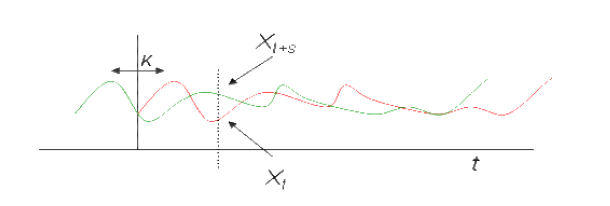
\includegraphics[scale=0.6]{graf17.png}\\
\textbf{Σχήμα 1.19:Τα ζεύγη της χρονοσειράς με τον εαυτό της μετατοπισμένο κατά s.}
\end{center}
Σαν συνάρτηση αυτοσυσχέτισης (ACF) ονομάζεται η συνάρτηση\\
$$ \rho_s\left(X\right)=\frac{\gamma_s\left(x\right)}{\gamma_0\left(x\right)}=\frac{\gamma_s}{\gamma_0}=\rho_s $$
$$ \rho_s=\frac{\sum_{i=1}^{N-s} \left(X\left(t_i\right)-\mu_X\right)\left(X\left(t_{i+s}\right)-\mu_X\right)}{\sum_{i=1}^{N} \left(X\left(t_i\right)
-\mu_X\right)^2} $$
όπου ο $ \mu_X$
ο μέσος της χρονολογικής σειράς.\\\\
Η συνάρτηση
 $$ \gamma_s \left(X\right)=Cov\left(Y_t,Y_{t+s}\right)=Cov\left(Y_{t-s},Y_t\right)=\gamma_s $$ ονομάζεται συνάρτηση αυτοδιασποράς (ACVF) μιας στάσιμης χρονολογικής σειράς.\\
Για τις παραπάνω συναρτήσεις ισχύουν τα εξής:\\
$$\gamma_0=\sigma^2, \quad \vert \gamma_s\vert \leq \gamma_0, \quad \gamma_s=\gamma_{-s}$$\\
$$ \rho_0=1,\quad \vert\rho_s\vert \leq 1,\quad \rho_s=\rho_{-s} $$\\

Η σημασία της συνάρτησης αυτοσυσχέτισης είναι πολύ μεγάλη, πρώτον γιατί δίνει το μέτρο της συσχέτισης των παρατηρήσεων – μετρήσεων οι οποίες απέχουν
κατά το χρονικό διάστημα s και δεύτερον γιατί δείχνει τόσο το βαθμό (ένταση) όσο
και το μήκος ή την χρονική διάρκεια της μνήμης της στοχαστικής διαδικασίας.
∆ηλαδή, εκφράζει κατά πόσο οι μετρήσεις με χρονική απόσταση s έχουν σχέση
μεταξύ τους. Με άλλα λόγια, η συνάρτηση αυτοσυσχετίσεως μας δείχνει κατά πόσο
το παρόν θυμάται το παρελθόν, και κατά πόσο το μέλλον θα επηρεαστεί από το παρόν.








%%%%%%%%%%%%%%% File ends here %%%%%%%%%%%%%%%%%%%%%%%%%%%%%%%%
\endinput
%%% Local Variables: 
%%% mode: latex
%%% TeX-master: "ptyxiakn"
%%% End: 
